\documentclass[../../main.tex]{subfiles}
\graphicspath{{\subfix{../../image/}}} % 指定图片目录,后续可以直接使用图片文件名。

% 例如:
% \begin{figure}[h]
% \centering
% \includegraphics{image-01.01}
% \caption{图片标题}
% \label{fig:image-01.01}
% \end{figure}
% 注意:上述\label{}一定要放在\caption{}之后,否则引用图片序号会只会显示??.

\begin{document}

\section{群}

\begin{definition}
令 $(S, \cdot)$ 是一个幺半群,$x \in S$。我们称 $x$ 是\textbf{可逆的},当且仅当
\begin{align*}
\exists y \in S, x \cdot y = y \cdot x = e
\end{align*}
其中 $y$ 被称为 $x$ 的\textbf{逆元},记作 $x^{-1}$。 
\end{definition}

\begin{proposition}[逆元存在必唯一]
令 $(S, \cdot)$ 是一个幺半群。假设 $x \in S$ 是可逆的,则其逆元唯一。也就是说,如果 $y, y' \in S$ 都是它的逆元,则 $y = y'$。
\end{proposition}
\begin{proof}
假设 $y, y'$ 都是 $x$ 的逆元。则 $y \cdot x = e$,$x \cdot y' = e$.从而
\begin{align*}
y = y \cdot e = y \cdot x \cdot y' = e \cdot y' = y' .
\end{align*}
\end{proof}

\begin{definition}[群]
令 $(G, \cdot)$ 是一个幺半群,若$G$ 中所有元素都是可逆的,则我们称$(G,\cdot)$是一个\textbf{群}.换言之,若 $\cdot$ 是 $G$ 上的一个二元运算,则我们称 $(G, \cdot)$ 是个\textbf{群},或 $G$ 对 $\cdot$ 构成群,当这个运算满足结合律,存在单位元,且每个元素具有逆元。再进一步展开来说,同样等价地,若 $\cdot$ 是 $G$ 上的一个二元运算,则我们称 $(G, \cdot)$ 是个\textbf{群},当
\begin{gather*}
\forall x, y, z \in G, x \cdot (y \cdot z) = (x \cdot y) \cdot z ,\\
\exists e \in G, \forall x \in G, x \cdot e = e \cdot x = x ,\\
\forall x \in G, \exists y \in G, x \cdot y = y \cdot x = e .
\end{gather*} 
\end{definition}

\begin{proposition}
令 $(G, \cdot)$ 是一个群,令 $x \in G$,则 $(x^{-1})^{-1} = x$。
\end{proposition}
\begin{proof}
方便起见,我们令 $y = x^{-1}$,于是有 $x \cdot y = y \cdot x = e$。我们要证明 $y^{-1} = x$,而这就是 $y \cdot x = x \cdot y = e$,显然成立。这就证明了逆元的逆元是自身.
\end{proof}

\begin{proposition}
令 $(G, \cdot)$ 是一个群,令 $x, y \in G$,则 $(x \cdot y)^{-1} = y^{-1} \cdot x^{-1}$。
\end{proposition}
\begin{proof}
我们利用定义来证明。一方面,利用广义结合律,$(x \cdot y) \cdot (y^{-1} \cdot x^{-1}) = e$;另一方面,同理可以得到另一边的等式$(y^{-1} \cdot x^{-1}) \cdot (x \cdot y) = e$,这就告诉我们 $(x \cdot y)^{-1} = y^{-1} \cdot x^{-1}$。 
\end{proof}

\begin{definition}\label{definition:群中元素负幂的定义}
设$(G,\cdot)$ 是一个群,且 $x\in G$。若 $n\in\mathbb{N}_1$,我们定义 $x^{-n}=(x^{-1})^n$,另外定义$x^0 = e$。 
\end{definition}

\begin{proposition}\label{proposition:关于元素幂的一些性质}
设$(G,\cdot)$ 是一个群,且 $x\in G$.则满足
\begin{enumerate}[(1)]
\item $x^{-n}=(x^{-1})^n=(x^n)^{-1}$,$\forall n\in\mathbb{Z}$.

\item $x^{m+n}=x^m\cdot x^n,\forall m,n\in \mathbb{Z}$ .

\item $x^{mn}=\left( x^m \right) ^n=\left( x^n \right) ^m,\forall m,n\in \mathbb{Z} .$
\end{enumerate}
\end{proposition}
\begin{proof}
\begin{enumerate}[(1)]
\item (i)当$n=0$时,结论显然成立.

(ii)当$n\in \mathbb{N}_1$时,只需证明$(x^{-1})^n=(x^n)^{-1}$即可.注意到
\begin{align*}
&x^n\cdot (x^{-1})^n=\left( \underset{n\text{个}}{\underbrace{x\cdots x}} \right) \cdot \left( \underset{n\text{个}}{\underbrace{x^{-1}\cdots x^{-1}}} \right) =e,
\\
&(x^n)^{-1}\cdot x^n=\left( \underset{n\text{个}}{\underbrace{x^{-1}\cdots x^{-1}}} \right) \cdot \left( \underset{n\text{个}}{\underbrace{x\cdots x}} \right) =e.
\end{align*}
故根据逆元的定义可知结论成立.

(iii)当$n$为负整数时,令$m=-n$,则$m\in \mathbb{N}_1$.从而我们只需证$x^m=(x^{-1})^{-m}=(x^{-m})^{-1}$即可.根据\hyperref[definition:群中元素负幂的定义]{定义\ref{definition:群中元素负幂的定义}}可得
\begin{align*}
&x^{-m}\cdot x^m=\left( x^{-1} \right) ^m\cdot x^m=\left( \underset{m\text{个}}{\underbrace{x^{-1}\cdots x^{-1}}} \right) \cdot \left( \underset{m\text{个}}{\underbrace{x\cdots x}} \right) =e,
\\
&x^m\cdot x^{-m}=x^m\cdot \left( x^{-1} \right) ^m=\left( \underset{m\text{个}}{\underbrace{x\cdots x}} \right) \cdot \left( \underset{m\text{个}}{\underbrace{x^{-1}\cdots x^{-1}}} \right) =e.
\end{align*}
故根据逆元的定义可知$x^m=\left( x^{-m} \right) ^{-1}$.
又由\hyperref[definition:群中元素负幂的定义]{定义\ref{definition:群中元素负幂的定义}}可知,$\left( x^{-1} \right) ^{-m}=\left( \left( x^{-1} \right) ^{-1} \right) ^m=x^m$.故结论成立.

\item 首先注意到,

(i)如果 $m,n\in\mathbb{N}_1$,则由\hyperref[corollary:满足结合律一定满足广义结合律的推论]{推论\ref{corollary:满足结合律一定满足广义结合律的推论}}就立刻得到这个性质。若 $m$ 或 $n$ 是 $0$,利用单位元的性质也是显然的。从而我们只需证明当$m,n$至少有一个小于0时,$x^{m+n}=x^m\cdot x^n$.故我们可以不失一般性,假设 $m<0$,记 $m'=-m$,则 $x^m = x^{-m'}=(x^{-1})^{m'}$。

(ii)若 $n<0$,记 $n'=-n$,则同理,$x^n=(x^{-1})^{n'}$,故 $x^{m + n}=(x^{-1})^{m'+n'}$,这里 $m',n'\in\mathbb{N}_1$,于是就有
\begin{align*}
x^{m+n}=(x^{-1})^{m' +n'}=\left( x^{-1} \right) ^{m'}\left( x^{-1} \right) ^{n'}=x^mx^n,
\end{align*}
因此得证了.

(iii)若 $0 < n < m'$,则 $x^{m + n}=x^{-(m'-n)}=(x^{-1})^{m'-n}$。而 $x^m\cdot x^n=(x^{-1})^{m'}\cdot x^n$.于是
\begin{align*}
&\quad \quad x^{m + n}=x^m\cdot x^n\\
&\Leftrightarrow (x^{-1})^{m' - n}=(x^{-1})^{m'}\cdot x^n\\
&\Leftrightarrow \underbrace{x^{-1}\cdots x^{-1}}_{m' - n\text{个}}= \left(\underbrace{x^{-1}\cdots x^{-1}}_{m'\text{个}}\right)\cdot x^n
\end{align*}
对上式两边左乘$x^{m' - n}$,得到
\begin{align*}
&\quad \quad x^{m + n}=x^m\cdot x^n
\Leftrightarrow \underbrace{x^{-1}\cdots x^{-1}}_{m' - n\text{个}}= \left(\underbrace{x^{-1}\cdots x^{-1}}_{m'\text{个}}\right)\cdot x^n
\\
&\Leftrightarrow x^{m' -n}\cdot \left( \underset{m' -n\text{个}}{\underbrace{x^{-1}\cdots x^{-1}}} \right) =x^{m' -n}\cdot \left( \underset{m' \text{个}}{\underbrace{x^{-1}\cdots x^{-1}}} \right) \cdot x^n
\\
&\Leftrightarrow \left( \underset{m' -n\text{个}}{\underbrace{x\cdots x}} \right) \cdot \left( \underset{m' -n\text{个}}{\underbrace{x^{-1}\cdots x^{-1}}} \right) =\left( \underset{m' -n\text{个}}{\underbrace{x\cdots x}} \right) \cdot \left( \underset{m' \text{个}}{\underbrace{x^{-1}\cdots x^{-1}}} \right) \cdot x^n
\\
&\Leftrightarrow e=\left( \underset{n\text{个}}{\underbrace{x^{-1}\cdots x^{-1}}} \right) \cdot x^n
\Leftrightarrow e=(x^n)^{-1}\cdot x^n
\end{align*}
上式最后一个等式显然成立,故此时结论成立.

(iv)若 $n\geq m'$,则$x^{m + n}=x^{n-m'}$。而 $x^m\cdot x^n=(x^{-1})^{m'}\cdot x^n$.于是
\begin{align*}
&\quad \quad x^{m+n}=x^m\cdot x^n
\\
&\Leftrightarrow x^{n-m'}=(x^{-1})^{m'}\cdot x^n
\\
&\Leftrightarrow \underset{n-m' \text{个}}{\underbrace{x\cdots x}}=\left( x^{-1} \right) ^{m'}\cdot \left( \underset{n\text{个}}{\underbrace{x\cdots x}} \right) 
\end{align*}
对上式两边右乘$(x^{-1})^{n-m'}$,得到
\begin{align*}
&\quad \quad x^{m+n}=x^m\cdot x^n\Leftrightarrow \underset{n-m' \text{个}}{\underbrace{x\cdots x}}=\left( x^{-1} \right) ^{m'}\cdot \left( \underset{n\text{个}}{\underbrace{x\cdots x}} \right) 
\\
&\Leftrightarrow \left( \underset{n-m' \text{个}}{\underbrace{x\cdots x}} \right) \cdot \left( x^{-1} \right) ^{n-m'}=\left( x^{-1} \right) ^{m'}\cdot \left( \underset{n\text{个}}{\underbrace{x\cdots x}} \right) \cdot \left( x^{-1} \right) ^{n-m'}
\\
&\Leftrightarrow \left( \underset{n-m' \text{个}}{\underbrace{x\cdots x}} \right) \cdot \left( \underset{n-m' \text{个}}{\underbrace{x^{-1}\cdots x^{-1}}} \right) =\left( x^{-1} \right) ^{m'}\cdot \left( \underset{n\text{个}}{\underbrace{x\cdots x}} \right) \cdot \left( \underset{n-m' \text{个}}{\underbrace{x^{-1}\cdots x^{-1}}} \right) 
\\
&\Leftrightarrow e=\left( x^{-1} \right) ^{m'}\cdot \left( \underset{m' \text{个}}{\underbrace{x\cdots x}} \right) \Leftrightarrow e=\left( x^{-1} \right) ^{m'}\cdot x^{m'}
\end{align*}
上式最后一个等式显然成立,故此时结论成立.

\item 先证$x^{mn}=(x^m)^n$.对$\forall m\in \mathbb{Z}$,固定$m$,对$n$使用数学归纳法.当$n=1$时,结论显然成立.假设当$n=k$时,结论成立,即$x^{mk}=\left( x^m \right) ^k$.则由(2)的结论可得
\begin{align*}
x^{m\left( k+1 \right)}=\left( x^m \right) ^{k+1}=\left( x^m \right) ^k\cdot x^m=\left( x^m \right) ^{k+1}.
\end{align*}
故由数学归纳法可知,$x^{mn}=(x^m)^n$,$\forall n\in \mathbb{Z}$.再由$m$的任意性可知$x^{mn}=(x^m)^n$,$\forall m,n\in \mathbb{Z}$.
同理可证$x^{nm}=(x^n)^m$,$\forall m,n\in \mathbb{Z}$.由于$x^{nm}=x^{mn}$,$\forall m,n\in \mathbb{Z}$.因此$x^{mn}=(x^m)^n=(x^n)^m$,$\forall m,n\in \mathbb{Z}$.
\end{enumerate}
\end{proof}

\begin{definition}[Abel群]
若 $(G, \cdot)$ 是一个群,我们称它是\textbf{Abel群},或\textbf{交换群},当该运算满足交换律,即
\begin{align*}
\forall x, y \in G, x \cdot y = y \cdot x
\end{align*} 
\end{definition}

\begin{example}[$\,\,$常见的群]
\begin{enumerate}
\item 我们称只有一个元素的群为\textbf{平凡群},记作${e}$.其中的二元运算是$e\cdot e=e$.
\item 常见的加法群有$(\mathbb{Z},+),$ $(\mathbb{Q},+),$ $(\mathbb{R},+),$ $(\mathbb{C},+)$等.这些加法群分别称为整数加群、有理数加群、实数加群、复数加群.
\item 常见的乘法群有$(\mathbb{Q}^\times,+),$ $(\mathbb{R}^\times,+),$ $(\mathbb{C}^\times,+)$等, 其中$\mathbb{Q}^\times=\mathbb{Q}\backslash {0}$,类似地定义其余两个集合.这些乘法群分别称为有理数乘群、实数乘群、复数称群.
\item 在向量空间中,$n$维欧式空间对加法构成群即$(\mathbb{R}^n,+)$.类似地$(\mathbb{C}^n,+),$ $(\mathbb{Q}^n,+),$ $(\mathbb{Z}^n,+)$也是群.对于这些群,单位元都是零向量,加法逆元则是对每个坐标取相反数,如$(x_1,\cdots,x_n)$的加法逆元是$(-x_1,\cdots,-x_n)$.
\item 所有的$m\times n$矩阵也对加法构成群,单位元都是零矩阵,加法逆元则是对每一项取相反数.对于$n\times n$的实矩阵加法群,我们记作$(M(n,\mathbb{R}),+)$,类似地我们将$n\times n$的复矩阵加法群记作$(M(n,\mathbb{C}),+)$.
\end{enumerate}
\end{example}
\begin{proof}
证明都是显然的.
\end{proof}

\begin{lemma}
令 $(S, \cdot)$ 是一个幺半群,令 $G$ 是其所有可逆元素构成的子集,则 $(G, \cdot)$ 是个群。
\end{lemma}
\begin{remark}
我们称呼幺半群中的可逆元素为 “\textbf{单位}”,因此 $G$ 是由所有该运算下的单位构成的集合(在这里甚至是群)。
\end{remark}
\begin{proof}
首先结合律完全继承自 $S$,不需要证明。而单位元是可逆的,因此 $e \in G$。剩下要证明 $G$ 中每个元素都有($G$ 中的)逆元,而这几乎是显然的。假设 $x \in G$,则 $x$ 是可逆元素,我们取 $y \in S$,使得 $x \cdot y = y \cdot x = e$(这里要注意我们只能首先保证 $y$ 在全集 $S$ 中)。接下来我们要证明 $y \in G$,即 $y$ 可逆,而这是显然的,因为 $x$ 正是它的逆。所以 $y \in G$。这样,就证明了 $(G, \cdot)$ 是个群.
\end{proof}

\begin{definition}[子群]
设$(G, \cdot)$ 是一个群,且 $H \subset G$。我们称 $H$ 是 $G$ 的\textbf{子群},记作 $H < G$,当其包含了单位元,在乘法和逆运算下都封闭,即
\begin{gather*}
e \in H ,\\
\forall x, y \in H, x \cdot y \in H ,\\
\forall x \in H, x^{-1} \in H.
\end{gather*} 
\end{definition}

\begin{proposition}[子群也是群]
令 $(G, \cdot)$ 是一个群。若 $H$ 是 $G$ 的子群,则 $(H, \cdot)$ 也是个群。
\end{proposition}
\begin{proof}
就二元运算的良定义性而言,子群第一个条件(封闭性)就满足了,这使得我们后面的谈论是有意义的。首先,结合律肯定满足,因为它是个子集。其次,根据子群的第二个条件,$e \in H$ 是显然的。再次,我们要证明每个 $H$ 中元素有 $H$ 中的逆元,而这是子群的第三个条件。
\end{proof}

\begin{corollary}[子群的传递性]
若$(G, \cdot)$ 是一个群,且$H<G$,$K<H$,则一定有$K<G$.因此我们可以将$H<G$,$K<H$简记为$K<H<G$.
\end{corollary}
\begin{proof}
证明是显然的.
\end{proof}

\begin{proposition}[子群的等价条件]\label{proposition:子群的等价条件}
$(H,\cdot)$是子群等价于
\begin{gather*}
e \in H,\\
\forall x, y \in H, x \cdot y^{-1} \in H .
\end{gather*}
\end{proposition}
\begin{proof}
设$(H,\cdot)$是子群。令 $x, y \in H$,利用逆元封闭性得到 $y^{-1} \in H$,再利用乘法封闭性得到 $x \cdot y^{-1} \in H$。

反过来,假设上述条件成立.令 $x \in H$,则 $e \cdot x^{-1} = x^{-1} \in H$,这证明了逆元封闭性。
接下来,令 $x, y \in H$,则利用逆元封闭性,$y^{-1} \in H$,故 $x \cdot (y^{-1})^{-1} = x \cdot y \in H$。这就证明了乘法封闭性。

综上,这的确是子群的等价条件。
\end{proof}

\begin{proposition}[子群的任意交仍是子群]\label{proposition:子群的任意交仍是子群}
设$G$是一个群, $(H_i)_{i\in I}$ 是一族 $G$ 的子群,则它们的交集仍然是 $G$ 的子群,即
\begin{align*}
\bigcap_{i\in I}N_i< G .
\end{align*}
\end{proposition}
\begin{proof}
首先,设$e$是$G$的单位元,则由子群对单位元封闭可知,$e\in N_i$,$\forall i\in I$.从而$e\in \bigcap_{i\in I}N_i.$

其次,对$\forall x,y\in \bigcap_{i\in I}N_i$,都有$x,y\in N_i$,$\forall i\in I$.根据子群对逆元封闭可知,$y^{-1}\in N_i$,$\forall i\in I$.于是再由子群对乘法封闭可知,$xy^{-1}\in N_i$,$\forall i\in I$.故$xy^{-1}\in \bigcap_{i\in I}N_i.$

综上,$\bigcap_{i\in I}N_i< G .$
\end{proof}

\begin{definition}[一般线性群]
我们对于那些 $n*n$ 可逆实矩阵构成的乘法群,称为\textbf{(实数上的)$n$ 阶一般线性群},记作 $(GL(n, \mathbb{R}), \cdot)$。由于一个矩阵可逆当且仅当其行列式不为零,因此
\begin{align*}
GL(n, \mathbb{R}) = \{A \in M(n, \mathbb{R}) : \det(A) \neq 0\}.
\end{align*} 
\end{definition}

\begin{definition}[特殊线性群]
我们将由那些行列式恰好是 $1$ 的 $n*n$ 实矩阵构成的乘法群称为\textbf{(实数上的)$n$ 阶特殊线性群},记作 $(SL(n, \mathbb{R}), \cdot)$,即
\begin{align*}
SL(n, \mathbb{R}) = \{A \in M(n, \mathbb{R}) : \det(A) = 1\}.
\end{align*} 
\end{definition}

\begin{proposition}
$(SL(n, \mathbb{R}), \cdot)$ 是个群。
\end{proposition}
\begin{proof}
根据定义,$SL(n, \mathbb{R})$ 首先是 $GL(n, \mathbb{R})$ 的子集,那么只要证明它是个子群即可。首先,乘法单位元单位矩阵的行列式恰好是 1(这也是为什么我们定义特殊线性群是行列式是 1 的矩阵构成的群的原因),这就证明了 $I \in SL(n, \mathbb{R})$($I = I_n$ 指的是 $n$ 阶单位矩阵)。另外,我们要证明 $SL(n, \mathbb{R})$ 在乘法下封闭。令 $A, B$ 是两个行列式为 1 的 $n*n$ 实矩阵。由于行列式满足 $\det(AB) = \det(A)\det(B)$,因此 $AB$ 的行列式也是 1,也就在特殊线性群中。这就证明了特殊线性群确实是个群。至于逆元封闭性,我们利用 $\det(A^{-1}) = \frac{1}{\det(A)}$。假设 $\det(A) = 1$,则 $\det(A^{-1}) = 1$,于是 $A^{-1} \in SL(n, \mathbb{R})$。综上,特殊线性群确实是个群。 
\end{proof}

\begin{definition}[群同态]
令 $(G, \cdot), (G', *)$ 是两个群,且 $f : G \to G'$ 是一个映射。我们称 $f$ 是一个\textbf{群同态},当其保持了乘法运算,即
\begin{align*}
\forall x, y \in G, f(x \cdot y) = f(x) * f(y).
\end{align*} 
\end{definition}

\begin{proposition}\label{proposition:群同态保持逆元和单位元}
若 $f : (G, \cdot) \to (G', *)$ 是一个群同态,则 $f(e) = e'$,$f(x^{-1}) = f(x)^{-1}$。
\end{proposition}
\begin{note}
也就是说,$f$ 不仅把乘积映到乘积,而且把单位元映到单位元,把逆元映到逆元。在这个意义下,实际上 $f$ 将所有群 $G$ 的 “信息” 都保持到了 $G'$ 上,包括单位元,乘法和逆元。至于结合律(或者更基础的封闭性),显然两边本来就有,就不必再提。
\end{note}
\begin{proof}
首先,因为 $e \cdot e = e$,所以利用同态的性质,$f(e) = f(e \cdot e) = f(e) * f(e)$。这时,两边同时左乘 $f(e)^{-1}$,就可以各约掉一个 $f(e)$,得到 $e' = f(e)$,这就证明了 $f$ 把单位元映到单位元。

另一方面,令 $x \in G$,则 $e' = f(e) = f(x \cdot x^{-1}) = f(x) * f(x^{-1})$。同理 $e' = f(x^{-1}) * f(x)$。于是由定义,$f(x^{-1})$ 就是 $f(x)$ 的逆元,即 $f(x^{-1}) = f(x)^{-1}$。这就证明了这个命题。 
\end{proof}

\begin{definition}[群同态的核与像]
令 $f : (G, \cdot) \to (G', *)$ 是一个群同态,则我们定义 $f$ 的\textbf{核}与\textbf{像},记作 $\ker(f)$ 与 $\mathrm{im}(f)$,分别为
\begin{gather*}
\ker(f) = \{x \in G : f(x) = e'\} \subset G ,\\
\mathrm{im}(f) = \{y \in G' : \exists x \in G, y = f(x)\} = \{f(x) : x \in G\} \subset G'.
\end{gather*} 
\end{definition}
\begin{note}
群同态的核与像示意图如下:
\begin{figure}[H]
\centering
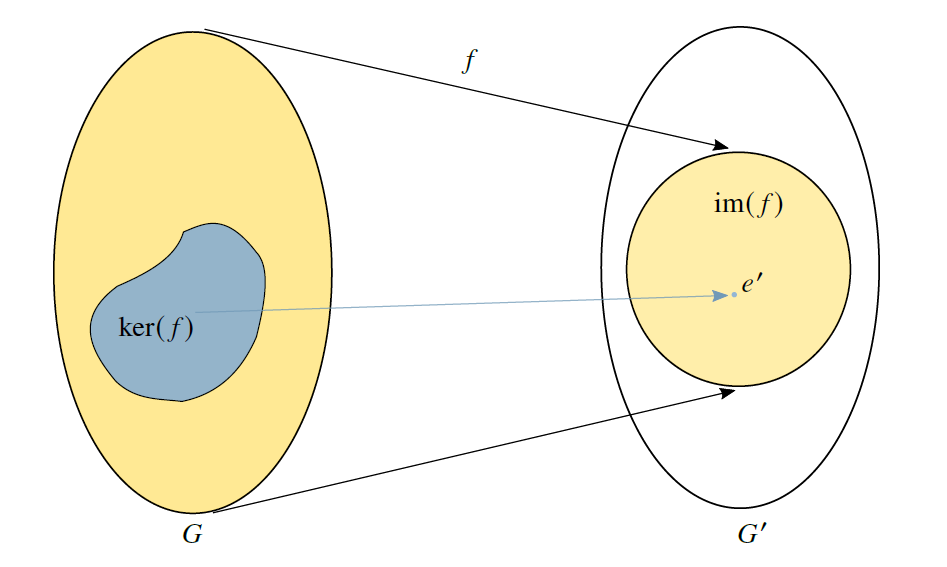
\includegraphics[scale=0.35]{群同态的核与像示意图.png}
\label{figure:群同态的核与像示意图}
\caption{群同态的核与像示意图}
\end{figure}
\end{note}


\begin{proposition}\label{proposition:群同态的核是定义域的子群,像是陪域的子群}
令 $f:(G,\cdot)\to (G',*)$ 是一个群同态,则核是定义域的子群,像是陪域的子群,即
\begin{align*}
\ker(f) < G,\quad
\mathrm{im}(f) < G'.
\end{align*}
\end{proposition}
\begin{proof}
先证明第一个子群关系。我们利用 $f(e)=e'$ 来说明 $e\in\ker(f)$。接着,设 $x,y\in\ker(f)$,只需证明 $xy^{-1}\in\ker(f)$。利用同态的性质,$f(xy^{-1}) = f(x)f(y)^{-1}=e'e'^{-1}=e'$,这就证明了 $xy^{-1}\in\ker(f)$。第一个子群关系得证。

再证明第二个子群关系。同样由于 $f(e)=e'$,我们有 $e'\in\mathrm{im}(f)$。接着,设 $y = f(x),y' = f(x')\in\mathrm{im}(f)$,只需证明 $yy'^{-1}\in\mathrm{im}(f)$。同样利用同态的性质,$yy'^{-1}=f(x)f(x')^{-1}=f(xx'^{-1})\in\mathrm{im}(f)$。第二个子群关系也得证。这样我们就证完了整个命题。
\end{proof}

\begin{example}
证明:$(SL(n,\mathbb{R}),\cdot)<(GL(n,\mathbb{R}),\cdot)$.
\end{example}
\begin{proof}
由\hyperref[proposition:行列是就是一个乘法群同态]{命题\ref{proposition:行列是就是一个乘法群同态}}可知,$\det : GL(n, \mathbb{R}) \to (\mathbb{R}^\times, \cdot)$ 是一个乘法群同态.注意到$\ker (det)=(SL(n,\mathbb{R}),\cdot)$,因此由\hyperref[proposition:群同态的核是定义域的子群,像是陪域的子群]{命题\ref{proposition:群同态的核是定义域的子群,像是陪域的子群}}可知,$(SL(n,\mathbb{R}),\cdot)=\ker (det)<(GL(n,\mathbb{R}),\cdot)$.
\end{proof}

\begin{definition}[满同态与单同态]
令 $f:(G,\cdot)\to (G',*)$ 是一个群同态,我们称 $f$ 是一个\textbf{满同态}当 $f$ 是满射,称 $f$ 是一个\textbf{单同态}当 $f$ 是单射。 
\end{definition}

\begin{proposition}\label{proposition:一个群同态是单的当且仅当核是平凡的}
令 $f:(G,\cdot)\to (G',*)$ 是一个群同态,则
\begin{enumerate}
\item $f$ 是一个单同态当且仅当 $\ker(f)=\{e\}$。也就是说,一个群同态是单的当且仅当核是平凡的。

\item $f$ 是一个满同态当且仅当 $ \mathrm{im}(f)=G'$。也就是说,一个群同态是满的当且仅当值域等于陪域。
\end{enumerate}
\end{proposition}
\begin{proof}
\begin{enumerate}
\item 假设 $f$ 是单的,那么因为 $f(e)=e'$,因此若 $f(x)=e'$,则利用单射的性质我们一定有 $x = e$,这就证明了核是平凡的。(这个方向是显然的)

另一个方向不那么显然。我们假设 $\ker(f)=\{e'\}$。假设 $x,x'\in G$,使得 $f(x)=f(x')$,我们只须证明 $x = x'$。在这里,我们同时右乘 $f(x')^{-1}$,得到 $f(x)f(x'^{-1})=f(xx'^{-1})=e'$。而因为核是平凡的,所以必须有 $xx'^{-1}=e$。接下来同时右乘 $x'$,我们就得到 $x = x'$。这就证明了这个命题.

\item 因为$f$是满同态,所以对$\forall a'\in G'$,都存在$a\in G$,使得$f(a)=a'.$故$a'\in \mathrm{im}(f)$.因此$G' \subset \mathrm{im}(f).$.又显然有$\mathrm{im}(f) \subset G'.$故$\mathrm{im}(f) = G'.$
\end{enumerate}
\end{proof}
\begin{note}
平凡群,满同态和单同态示意图如下:
\begin{figure}[H]
\centering
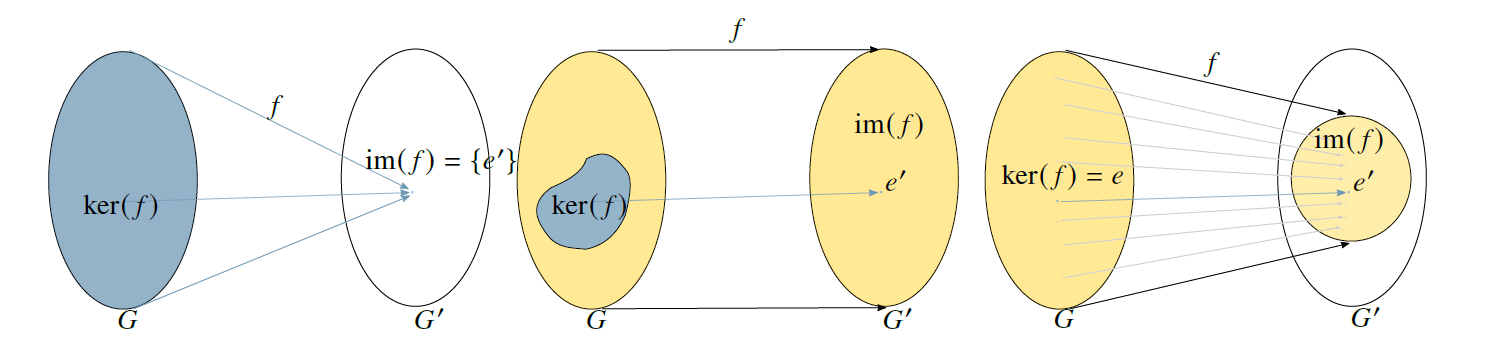
\includegraphics[scale=0.4]{平凡群,满同态和单同态示意图.png}
\label{figure:平凡群,满同态和单同态示意图}
\caption{平凡群,满同态和单同态示意图}
\end{figure}
\end{note}


\begin{example}\label{example:行列是就是一个乘法群同态}
证明:$\det : GL(n, \mathbb{R}) \to (\mathbb{R}^\times, \cdot)$ 是一个乘法群同态,并且是满同态,$\ker (\det)=SL(n, \mathbb{R}).$
\end{example}
\begin{proof}
设 \(A, B \in GL(n, \mathbb{R})\),则由行列式的 Laplace 定理可知 \(\det(AB) = \det(A)\det(B)\)。故 \(\det\) 是群同态。

任取 \(a \in \mathbb{R}^{\times}\),令 \(C = \begin{pmatrix}
a & & & \\
& 1 & & \\
& & \ddots & \\
& & & 1
\end{pmatrix}\),则 \(C \in GL(n, \mathbb{R})\) 并且 \(\det(C) = a\)。故 \(\det\) 是满同态。

一方面,任取 \(N \in SL(n, \mathbb{R})\),则 \(\det(N) = 1\),从而 \(N \in \mathrm{ker}(\det)\)。于是 \(SL(n, \mathbb{R}) \subset \mathrm{ker}(\det)\)。另一方面,任取 \(M \in \mathrm{ker}(\det)\),则 \(\det(M) = 1\),从而 \(M \in SL(n, \mathbb{R})\)。于是 \(\mathrm{ker}(\det) \subset SL(n, \mathbb{R})\)。故 \(\mathrm{ker}(\det) = SL(n, \mathbb{R})\)。 
\end{proof}

\begin{definition}[群同构]
令 $f:(G,\cdot)\to (G',*)$ 是一个映射,我们称 $f$ 是一个\textbf{群同构},当 $f$ 既是一个双射,又是一个群同态。简单来说,同构就是双射的同态。
\end{definition}

\begin{proposition}[群同构的逆也是群同构]
若 $f:(G,\cdot)\to (G',*)$ 是一个群同构,则 $f^{-1}$ 也是群同构。
\end{proposition}
\begin{proof}
因为 $f^{-1}$ 也是双射,所以我们只须证明 $f^{-1}$ 是群同态。令 $x',y'\in G'$,设 $x' = f(x),y' = f(y)$。则 $x'*y' = f(x\cdot y)$,$x=f^{-1}(x'),y=f^{-1}(y')$,故 $f^{-1}(x'*y')=x\cdot y = f^{-1}(x')\cdot f^{-1}(y')$。这就完成了证明。 
\end{proof}

\begin{definition}[两个群的直积]
令 $(G,\cdot_1),(G',\cdot_2)$ 是两个群,我们记$(G\times G',*)$为$(G,\cdot_1)$和$(G',\cdot_2)$的\textbf{直积}.满足对于 $(x,y),(x',y')\in G\times G'$,有
\begin{align*}
(x,y)*(x',y')=(x\cdot_1 x',y\cdot_2 y').
\end{align*}
\end{definition}

\begin{proposition}[两个群的直积仍是群]\label{proposition:两个群的直积仍是群}
若 $(G,\cdot_1),(G',\cdot_2)$ 是两个群,则它们的直积 $(G\times G',*)$ 还是一个群。
\end{proposition}
\begin{proof}
封闭性:因为 $G$ 在 $\cdot_1$ 下封闭,$G'$ 在 $\cdot_2$ 下封闭,而 $G\times G'$ 的元素乘积是逐坐标定义的,则 $G\times G'$ 在 $* = (\cdot_1,\cdot_2)$ 下也是封闭的。

结合律:同样,逐坐标有结合律,故整体也有结合律。

单位元:设$e,e'$分别是$(G,\cdot_1),(G',\cdot_2)$的单位元,则不难想象,$(e,e')$ 是直积的单位元。对于任意 $(x,y)\in G\times G'$,我们有 $(x,y)*(e,e')=(x\cdot_1 e,y\cdot_2 e')=(x,y)$,另一边也是同理,这就证明了 $(e,e')$ 是直积的单位元。

逆元:对于任意 $(x,y)\in G\times G'$,设$x^{-1},y^{-1}$分别是$x,y$的逆元,则同样不难想象,$(x^{-1},y^{-1})$ 是 $(x,y)$ 的逆元。 
\end{proof}

\begin{definition}[一族群的直积]
令 $(G_i,\cdot_i)_{i\in I}$ 是一族群,其中 $I$ 是一个指标集。我们记它们的\textbf{直积}为 $(\prod_{i\in I}G_i,*)$.满足对于 $(x_i)_{i\in I},(y_i)_{i\in I}\in\prod_{i\in I}G_i$,有
\begin{align*}
(x_i)_{i\in I}*(y_i)_{i\in I}=(x_i\cdot_i y_i)_{i\in I}.
\end{align*}
\end{definition}

\begin{proposition}[一族群的直积仍是群]
若 $(G_i,\cdot_i)_{i\in I}$ 是一族群,则它们的直积 $(\prod_{i\in I}G_i,*)$ 还是一个群。  
\end{proposition}
\begin{note}
最经典的例子就是通过 $n$ 个实数加群 $(\mathbb{R},+)$ 直积得到的 $(\mathbb{R}^n,+)$。
\end{note}
\begin{proof}
证明与\hyperref[proposition:两个群的直积仍是群]{命题\ref{proposition:两个群的直积仍是群}}同理.故我们只列出一些重点。封闭性与结合律是显然的。单位元是 $(e_i)_{i\in I}$,而 $(x_i)_{i\in I}$ 的逆元是 $(x_i^{-1})_{i\in I}$。 
\end{proof}


\begin{definition}[投影映射]
若 $(G_i,\cdot_i)_{i\in I}$ 是一族群,$j\in I$ 是任意指标,我们定义映射到指标 $j$ 的\textbf{投影映射}为
\begin{align*}
p_j:\prod_{i\in I}G_i&\to G_j.
\end{align*}
对于 $(x_i)_{i\in I}$,我们称$p_j((x_i)_{i\in I})=x_j$为$(x_i)_{i\in I}$的\textbf{投影}.
\end{definition}

\begin{proposition}[投影映射是群同态]\label{proposition:投影映射是群同态}
若 $(G_i,\cdot_i)_{i\in I}$ 是一族群,$j\in I$ 是任意指标,则投影映射 $p_j:\prod_{i\in I}G_i\to G_j$ 是个群同态。
\end{proposition}
\begin{proof}
令 $(x_i)_{i\in I},(y_i)_{i\in I}\in\prod_{i\in I}G_i$,则
\begin{gather*}
p_j((x_i)_{i\in I})=x_j,\quad p_j((y_i)_{i\in I})=y_j\\
p_j((x_i)_{i\in I}*(y_i)_{i\in I})=p_j((x_i\cdot_i y_i)_{i\in I})=x_j\cdot_j y_j = p_j((x_i)_{i\in I})\cdot_j p_j((y_i)_{i\in I}).
\end{gather*}
\end{proof}







\end{document}